\documentclass{alex_hü}

\name{Alexander Helbok}
\course{PS Physik}
\hwnumber{7}

\begin{document}
	\renewcommand{\labelenumi}{\alph{enumi})}
	
	
	\section*{75. Schwerpunkt}
	\begin{enumerate}
		\item $ $
		\begin{multicols}{2}
			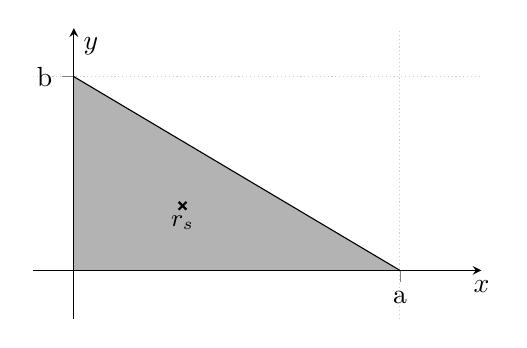
\begin{tikzpicture}
				\begin{axis}[
					width=207pt,
					height=150pt,
					axis lines=center,
%					y axis line style={thick},
					tick align=outside,
					xmin=-0.25,xmax=2.5,ymin=-0.25,ymax=1.25,
					xlabel style={below},
					xtick = {2}, ytick = {1},
					xticklabels={a},
					yticklabels={b},
					xlabel=$x$,
					ylabel=$y$,
					grid=major,
					grid style={thin,densely dotted,black!20},
					%legend columns=2,
					legend style={at={(axis description cs:1,0.35)},anchor=east}]
					\fill[fill=gray, opacity=0.6] (0,0)--(2,0)--(0,1);
					\path[draw] (0,0)--(2,0);
					\path[draw] (2,0)--(0,1);
					\path[draw] (0,1)--(0,0);
						\addplot [thick, mark=x]
					plot coordinates {
						(2/3,1/3)};
					\node[below] at (2/3,1/3) {\small$ r_s $};
				\end{axis}
			\end{tikzpicture}\\
			\columnbreak
			\begin{flalign*}
				\vec{r}_s &= \vector{x_s\\ y_s} &&\\
				dA &= l(y)*dy &&\\
				l(y) &= a (1 - \tfrac{y}{b}) &&\\
				y_s &= \tfrac{1}{A} \int_{0}^{b} l(y) * y \,dy = \tfrac{2}{ab} \int_{0}^{b} a (1 - \tfrac{y}{b}) y \,dy  &&\\
				y_s &= \tfrac{1}{3}\ b &&
			\end{flalign*}
		\end{multicols}
		Für $ x_s $ wird das Koordinatensystem gedreht $ \Rightarrow $ Formeln werden wiederverwendet
		\begin{flalign*}
			x_s &= \tfrac{1}{3}\ a \sigma\Sigma\varsigma &&\\
			\vec{r}_s &= \dl{\tfrac{1}{3} \vector{a\\ b}} &&
		\end{flalign*}
		\item $  $
		\begin{multicols}{2}
			\begin{tikzpicture}
				\begin{axis}[
					width=207pt,
					height=150pt,
					axis lines=center,
					%					y axis line style={thick},
					tick align=outside,
					xmin=-2.5,xmax=2.5,ymin=-0.25,ymax=2,
					xlabel style={below},
					xtick = {-2,-1,1,2}, ytick = {1.5},
					xticklabels={$-a_1$,$-a_2$,$a_2$,$a_1$},
					yticklabels={,},
					xlabel=$x$,
					ylabel=$y$,
					grid=major,
					grid style={thin,densely dotted,black!20},
					%legend columns=2,
					legend style={at={(axis description cs:1,0.35)},anchor=east}]
					\addplot[draw, name path=f] (2,0)--(1,1.5)--(-1,1.5)--(-2,0);
					\addplot[draw, dashed] (-1,0)--(-1,1.5);
					\addplot[draw, dashed] (1,0)--(1,1.5);
					\addplot[name path=g] {0};
					\addplot[gray, opacity=0.6] fill between[of=f and g, soft clip={domain=-2:2}];
					\addplot [thick, mark=x, only marks]
					plot coordinates {
						(0,1/2)(0,0.75)};
					\node[left] at (0,0.75) {\small$ r_{s_1} $};
					\node[right] at (0,1/2) {\small$ r_{s_2} $};
					\node[above left] at (0,1.5) {b};
				\end{axis}
			\end{tikzpicture}\\
			\columnbreak
			\begin{flalign*}
				x_s &= 0\quad \text{ (Symmetrie)} &&\\
				l(y) &= \tfrac{a_2-a_1}{b}\ y + a_1 &&\\
				y_s &= \tfrac{1}{A} \int_{0}^{b} l(y) * y \,dy = \tfrac{1}{A} \int_{0}^{b} \tfrac{a_2-a_1}{b}\ y + a_1 * y \,dy  &&\\
				y_s &= \tfrac{1}{3}\ b\ \tfrac{a_1 + 2a_2}{a_1 + a_2} &&\\
				\vec{r}_s &= \dl{\vector{0\\ \tfrac{1}{3}\ b\ \tfrac{a_1 + 2a_2}{a_1 + a_2}}} &&\\
			\end{flalign*}
		\end{multicols}
		\begin{minipage}{0.5\textwidth}
			Für $ a_1 = a_2 $
			\begin{flalign*}
				\vec{r}_{s_1} &= \vector{0\\ \tfrac{1}{3}\  b\ \tfrac{a_1 + 2a_1}{a_1 + a_1}} &&\\
				\vec{r}_{s_1} &= \dl{\vector{0\\ \tfrac{1}{2}\  b\ }} &&\\
			\end{flalign*}
		\end{minipage}
		\begin{minipage}{0.5\textwidth}
			Für $ a_2 = 0 $
			\begin{flalign*}
				\vec{r}_{s_2} &= \vector{0\\ \tfrac{1}{3}\ b\ \tfrac{a_1 + 2*0}{a_1 + 0}} &&\\
				\vec{r}_{s_2} &= \dl{\vector{0\\ \tfrac{1}{3}\  b\ }} &&\\
			\end{flalign*}
		\end{minipage}
	\end{enumerate}
	
	\section*{76. Anheben eines Seils}
	\begin{enumerate}
		\item
		\begin{flalign*}
			F(y) &= \dl{\tfrac{mgy}{l}} &&
		\end{flalign*}
		\item
		\begin{flalign*}
			W &= \int_{0}^{l} F(y) \,dy = \tfrac{mg}{l} \int_{0}^{l} y \,dy &&\\
			W &= \dl{\tfrac{mgl}{2}} &&
		\end{flalign*}
		\item $ m = \rho r^2\pi l $
		\begin{flalign*}
			x_s &= 0\quad \text{ (Mittelpunkt vom Seil)} &&\\
			y_s &= \tfrac{1}{m} \int_{0}^{l} \rho r^2\pi * y \,dy = \tfrac{\rho r^2\pi}{m} \int_{0}^{l} y \,dy &&\\
			y_s &= \tfrac{\rho r^2\pi}{m} * \tfrac{l^2}{2} = \tfrac{l}{2} &&\\
			\vec{r}_s &= \dl{\vector{0\\ \tfrac{l}{2}}} &&\\[2ex]
			E_{pot} &= g \int_{0}^{l} \rho r^2\pi * y \,dy = g*\rho r^2\pi \int_{0}^{l} y \,dy &&\\
			E_{pot} &= \tfrac{\rho r^2\pi gl^2}{2} = \dl{\tfrac{mgl}{2}} &&
		\end{flalign*}
		\item $ W $ stellt die Energieumwandlung/übertragung dar. Im Fall des Seils, welches zu Beginn 0 und am ende $ E_{pot} $ Energie besitzt, wird mittels Arbeit $ E_{pot} - 0 = E_{pot} $ zugeführt. Demnach gilt $ W = E_{pot} $
	\end{enumerate}
	
	\section*{77. Kette auf schiefer Ebene}
		\begin{multicols}{2}
			\begin{tikzpicture}
				\tikzmath{\x = 1.9; \y = 0.9; \a = -46.5; \w = 2.2; \e = 1;}
				\begin{axis}[
					width=207pt,
					height=150pt,
					axis lines=center,
					%y axis line style={thick},
					tick align=outside,
					xmin=0,xmax=4,ymin=0,ymax=2,
					xlabel style={below},
					xtick = {3}, ytick = {1},
					xticklabels={$ C $},
					yticklabels={$ A $},
					xlabel=$x$,
					ylabel=$y$,
					grid=major,
					grid style={thin,densely dotted,black!20},]
					\addplot[draw, name path=f] (3,0)--(1.75,1)--(0,1);
					\addplot[draw, thick, dashed] (1.75,1.03)--(2.5,0.45);
					\addplot[draw, thick, dashed] (1,1.03)--(1.75,1.03);
					\addplot[name path=g] {0};
					\addplot[gray, opacity=0.6] fill between[of=f and g, soft clip={domain=0:3}];
					\node[below left] at (1.75,1) {\small$ B $};
					\node[below] at (1,1) {\small$ D $};
					\draw (2.48,0.42) arc (132:180:0.6);
					\node[above] at (2.55,0) {\small$\alpha$};
%					
					\draw (1,1.2)--(1,1.3);
					\draw (1.75,1.2)--(1.75,1.3);
					\node at (1.4,1.25) {\tiny{$ L\!-\!a $}};
					\addplot [<-,  black] coordinates { (1,1.25) (1.2,1.25)};
					\addplot [->,  black] coordinates { (1.6,1.25) (1.75,1.25)};
%					
					\node[rotate=\a] at (\x+0.375,\y) {\tiny{$ a $}};
					\addplot [<-,rotate around={\a:(\x+0.375,\y)}, black] coordinates { (\x-0.1,\y) (\x+0.29,\y)};
					\addplot [->, rotate around={\a:(\x+0.375,\y)}] coordinates { (\x+0.5,\y) (\x+0.85,\y)};
					\draw[rotate around={\a:(\x+0.375,\y)}] (\x-0.1,\y-0.05)--(\x-0.1,\y+0.05);
					\draw[rotate around={\a:(\x+0.375,\y)}] (\x+0.85,\y-0.05)--(\x+0.85,\y+0.05);
%					
					\node[rotate=\a] at (\w+0.375,\e) {\tiny{$ L $}};
					\addplot [<-,rotate around={\a:(\w+0.375,\e)}, black] coordinates { (\w-0.2,\e) (\w+0.29,\e)};
					\addplot [->, rotate around={\a:(\w+0.375,\e)}] coordinates { (\w+0.5,\e) (\w+1.5,\e)};
					\draw[rotate around={\a:(\w+0.375,\e)}] (\w-0.2,\e-0.05)--(\w-0.2,\e+0.05);
					\draw[rotate around={\a:(\w+0.375,\e)}] (\w+1.5,\e-0.05)--(\w+1.5,\e+0.05);
%					
					\node [rotate=270] at (3.575,0.5) {\tiny\( L\sin(\alpha) \)};
					\draw (3.5,1) -- (3.65,1);
					\addplot [<-] coordinates {(3.575,1) (3.575,0.75)};
					\addplot [->] coordinates {(3.575,0.25) (3.575,0)};
				\end{axis}
			\end{tikzpicture}\\
			\columnbreak
			\begin{flalign*}
				t_0 &= \text{ start }; \quad t_1 = \text{ wenn } a = L \\[2ex]
				E_{pot}(t_0) &= g \left(m\ \tfrac{L-a}{L}\right) L\sin(\alpha) + g \left(m\ \tfrac{a}{L}\right) \left( L - \tfrac{a}{2} \right) \sin(\alpha) &&\\
				&= gm\sin(\alpha) \left( L - \tfrac{a^2}{2L} \right) &&\\
				E_{ges}(t_0) &= E_{pot}(t_0) &&\\[2ex]
				E_{pot}(t_1) &= mg\ \tfrac{L\sin(\alpha)}{2} &&\\
				E_{kin}(t_1) &= E_{ges}(t_0) - E_{pot}(t_1) &&\\[2ex]
				\tfrac{mv^2}{2} &= gm\sin(\alpha) \left( L - \tfrac{a^2}{2L} \right) - mg\ \tfrac{L\sin(\alpha)}{2} &&\\
				v &= \dl{\sqrt{g\sin(\alpha) \left(L - \tfrac{a^2}{L}\right)}} &&
			\end{flalign*}
		\end{multicols}
	
\end{document}